\chapter{Implementation of RoboMission}
\label{chap:implementation-of-robomission}

The first part of this chapter describes general aspects of the implementation,
such as used technologies and overall architecture of frontend and backend.
The second part presents a few selected details that are specific to the created system.

\section{System Architecture}

The application uses a standard client-server architecture,
with a fat frontend client communicating with server backend via REST API.
In addtion to the fronend app and backend service,
there are two other parts of the system:
scheduled jobs, which run periodically every night (e.g. metrics computation),
and tools for offline analysis of collected data
(jupyter notebook templates and helper functions).  % TODO: specify "helper functions"
% TODO: ref/cite human-in-the-loop principle
% TODO: other potential parts (future):
% - tasks/content management tools (CLI+browser)
% - simulations (CLI+browser)

% TODO: consider to include FE and BE sections below as subsections of this section

TODO: diagram of overall architecture (client-server, communication)

\section{Used Technologies}

Table \ref{tbl:technologies} shows overview of the tehcnologies used
in the project at the beginning of 2018.
Note that they are gradually evolving, either to meet new requirements,
or simply to replace old technologies with newer ones.
This is especially true for frontend, where the tools and best practices
are evolving rapidly.
When this project started in 2015,
we used several at that time popular technologies
(AngularJS, Bootstrap, bower, grunt)
which became obsolete during next 2 years,
so we replaced them by newer ones.
Many technologies were introduced naturally as the projects grew,
e.g. Django Rest Framework for REST API,
or redux-saga for cleaner handling of asynchronous side-effects
(instead of the originally used redux-thunk).


\begin{table}[h]
\begin{center}
\begin{tabular}{l l l}
\toprule
Area & Technology & Main Reason  \\
\midrule
Version control & git, GitHub & easy to use \\
Custom commands & make + django, npm & easy to use \\
Project management & GitHub (issues, project board) & easy to use \\
% Monitoring & Google Analytics & widely-used \\
\hline
\textbf{Backend} & Python 3 & concise, high-level \\
Dependencies & pip & easy to use \\
Environment & virtualenv[wrapper] & easy to use \\
Unit tests & pytest & concise, readable \\
Web framework & Django & feature-complete, well-documented \\
REST API & Django Rest Framework & feature-complete, well-documented \\
Database & PostgreSQL & widely used \\
Web server & Nginx + Gunicorn & widely used \\
Scheduled jobs & cron (+ django-crontab) & standard tool \\
Data Export & Django Rest Pandas & tranformations before export \\
\hline
\textbf{Frontend} & ES6 & concise and readable code \\
Dependencies & npm & easy to use \\
Bundling & webpack & feature-complete, widely used \\
Compling & babel & feature-complete, widely used \\
State & redux  & predictable behavior, testability \\
Side effects & redux-sagas  & readability, testability \\
Views & React & declarativness, reausability \\
Design (UI) & Material-UI & looks good \\
HTTP client & axios & based on promises \\
Code Blocks & Blockly & well-tested \\
Parsing & PEG JS & declarative rules \\  %(Parsing expression grammar) \\
Interpretation & JS-interpreter & stepping, custom hooks \\
Localization & react-intl & single place for all messages \\
\hline
\textbf{Analysis} & jupyter, pandas, sklearn & interactivity, high-levelness \\
Plotting & matplotlib, seaborn & powerful; results look good \\
%Machine learning & sklearn & powerful \\
%\hline
%\textbf{Analysis} & Python 3 & high-level, widely used \\
%Documents & jupyter notebook & interactivity \\
%DataFrames & pandas & feature-complete, well-documented \\
%Plotting & matplotlib, seaborn & powerful, looks good \\
%Machine learning & sklearn & powerful \\
\bottomrule
\end{tabular}
\end{center}
\caption{%
  Overview of main technologies used in the project. %
  The \emph{Reason} briefly explains why we have chosen the particular technoglogy
  (not why we have covered the area at all).}
\label{tbl:technologies}
\end{table}

\section{Frontend}

The frontend is a single page application with redux-architecture,
which means that there is a single state (model) storing all application data,
all the only way the state can be changed is by dispatching actions.
Each part of state then defines its reducer,
which is a pure function that takes previous state, action, and returns a new state.

TODO: redux-architecture diagram (specifically for our app)

TODO: show how the flow of events is easier to reason about in React+Redux (than in Angular)

\subsection{React Components}

\begin{itemize}
\item mostly declarative - simple mental model: rebuilding from scratch every time anything change -> less error prone
\item reusability -> use of single component on many places in different contexts,
  or even outside the app (use space-world for ai-search-workshop)
\item example from our codebase (code, image)
\end{itemize}

\subsection{Asynchronous Side Effects}

Frontend applications are usually full of asynchronous side effects
(e.g. fetching data from server, wating for user actions).
Many ways to handle them were proposed.
The most basic one are callbacks --
asychronous function takes a function (``callback'') as a parameter
and calls it once the asynchronous action is resolved.

(TODO: mention/explain promises -- advantage: very explicit; clean error
handling; show example for data fetching)

However, both callbacks and promises become awkward for expressing complex
asynchronous flows, such as visualizing code execution,
leading to unreadable ``callback hell''. % TODO: ref for callback hell
Sagas provide an alternative way of handling asynchronous effects using generators.
Instead of performing asynchronous effects directly, sagas yield
descriptions of such effects.
As an example, there is a saga responsible for processing
submitted feedback.
Note that while the code contains many asynchronous effects,
it can be read nearly as easy as standard linear synchronous code.

% TODO: insert comments in the code
% TODO: mention other advantage of sagas - great testability
% TODO: also mention new async-await concept

\begin{lstlisting}[language=ES6]
// Generator for single submit-feedback request
function* submitFeedback(action) {
  const { text, email } = action.payload;
  // Asynchronous request to get a value from state
  const url = yield select(getFeedbackUrl);
  try {
    // Asynchronous request to post data to server
    yield call(api.sendFeedback, url, text, email);
    // Asynchronous request to dispatch a new action
    yield put(actions.submitFeedback.success());
  }
  catch (error) {
    const { fieldErrors } = error;
    yield put(
      actions.submitFeedback.failure(fieldErrors));
  }
}
\end{lstlisting}


% TODO: add code samples for each concept (react component + image, reducer, saga)
% TODO(optional): awesome ES6 (example from our code)
% TODO(Material Design): example of our component + code

\begin{itemize}
\item TODO: (below) parsing task source, space world, robo code (PEG grammars)
\item TODO: Blockly
\item TODO: interpretation: saga + JS-interpreter
\end{itemize}

\section{Backend}

\begin{itemize}
\item Django, Django Rest Framework, (+ many small libraries, such as Django Rest Pandas)
\item django apps (python packages): learn, monitoring
\item models (...), serializers, views, services/use cases/core
\item data export
\item monitoring app, metrics computation
\item generators (e.g. metric computation)
\end{itemize}


\section{Tasks Description}

Each task is described by a single file in a restricted markdown format,
containing name, category, setting and solution.
The high-level grammar for task description looks like this:

\begin{lstlisting}
# <name>
[- option: value]*

## Setting
```
<SpaceWorld>
```
[- option: value]*

## Solution
```
<RoboCode>
```
\end{lstlisting}

Currently, there is one mandatory top-level option (task category)
adn two optional setting options (length, energy).
(TBA: ref to example below; ref to 2 subparts - SpaceWorld grammar, RoboCode grammar)
% [consider] Markdown files are then parsed and loaded into DB by a single command.

Task sources in markdown have several advantages:
it is human readable,
each change is version-controlled,
and the task can be edited easily in any text editor.
However, it is more convenient to use online task editor (REF to task editor fig),
unless it is a really minor modification, or unless one wants to change multiple tasks at once.

% [consider]
% - Localized task names are not part of the task source,
% because all localized messages live on the same place in a single file on FE.
% - PEG grammar for parsing
% - internal represenation (DB model and its serializers for FE and for CSV exports)


Example of complete task source (for rendered task see figure \ref{fig:robomission-task1}. TBA: show rendered task and its source side by side)

\begin{lstlisting}
# turning-left
- category: moves

## Setting

```
|bM|b |b |bM|b |
|kA|k |kM|k |kA|
|k |k |kA|kM|k |
|kM|k |kS|k |kA|
```

## Solution

```python
left()
fly()
fly()
```
\end{lstlisting}


\subsection{SpaceWorld Grammar}

Each SpaceWorld is described by a simple human-readable string. (TBA: ref to example below)
Each line describes one row of the grid
and is split by pipes (``|'') into fields.
Each field starts with a lower-cased letter denoting color of the field
(b -- blue, r -- red, k -- black, etc.),
followed by an optional upper-case letter denoting an object
(A -- asteroid, M -- meteoroid, W -- wormhole, S -- spaceship, etc.).
For example ``bA'' is a blue field with an asterorid.


\begin{figure}[h]
\begin{center}
\begin{subfigure}{.4\textwidth}
\centering
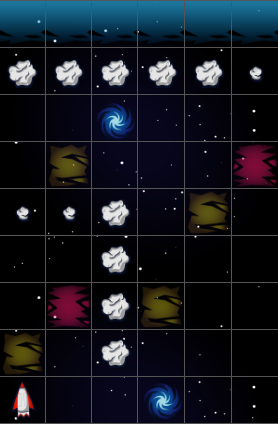
\includegraphics[width=.9\textwidth]{img/spaceworld}
\end{subfigure}
\begin{subfigure}{.36\textwidth}
\centering
{\lstset{numbers=none}
\begin{lstlisting}
|b |b |b |b |b |b |
|kA|kA|kA|kA|kA|kM|
|k |k |kW|k |k |k |
|k |y |k |k |k |r |
|kM|kM|kA|k |y |k |
|k |k |kA|k |k |k |
|k |r |kA|y |k |k |
|y |k |kA|k |k |k |
|kS|k |k |kW|k |k |
\end{lstlisting}}
\end{subfigure}
\end{center}
\caption{Example of Space World with its source code. TODO: Describe letters; consider replacing code listing with a screenshot from task editor with code highlighting}
\label{fig:spaceworld-source}
\end{figure}


\section{RoboCode}

RoboCode is a language based on Python that is used in task sources for solutions.
It is also meant to be used in more advanced levels as the transitional phase
from block-based to text-based programming.
The requirements for the language are following:
\begin{itemize}
\item easy for beginners, understandable without previous knowledge,
\item conciseness (short, but readable programs),
\item matching Blockly blocks closely (for easy transition from Blockly),
\item matching Python closely (for easy transition to Python).
\end{itemize}

\subsection{Syntax and Semantic}
\label{sec:syntax-semantic}

% TODO[consider] note on mixing lexer+parser+some semantic analysis
% (which is partially convenient, partially confusing)

There are four commands for performing actions:
\begin{lstlisting}
fly()
left()
right()
shoot()
\end{lstlisting}
Each action is combined with moving one row forward.
The movement takes place after the action, with the exception of left and right turning actions, where the movement and the action happen simultaneously,
i.e. the spaceship flies diagonally to the left or to the right.
% TODO: Rephrase. Is confusing, because the general statement ("movement takes
% place after the action") is only relevant for shoot(), and all the other
% commands are special cases.

Loops and conditional statements are same as in the Python,
with the notable exception of the repeat loop,
which was simplified to the form matching a corresponding
Blockly block, which is easier to understand by beginners:
% TODO: ass robocode highlighting
\begin{lstlisting}
repeat 4:
    fly()
\end{lstlisting}

Tests inside while-loops and if-statements are limited to the following forms
(again in order to match the respective Blockly blocks):
\begin{lstlisting}
position() [==|!=|>|<|>=|<=] [1..6]
color() [==|!=] ['r'|'g'|'b'|'y'|'k']
<test> [and|or] <test>
\end{lstlisting}
The letters in the color-test have the same meaning as in the space world description,
('r' for red, 'g' for green, etc.)


\subsection{RoboAST}

\begin{table}[h]
\begin{center}
\begin{tabular}{l l l}
\toprule
Name & Form & Usage  \\
\midrule
RoboCode     & textual (Python-like) & sample solutions in task sources  \\
MiniRoboCode & compact string & logging, storing in DB, analysis  \\
RoboBlocks   & Blockly blocks & code editor for students  \\
RoboJS       & textual (JavaScript) & interpretation in browser  \\
RoboAST      & json (AST) & common intermediate representation \\
\bottomrule
\end{tabular}
\end{center}
\caption{Different code representaions used within the system.}
\label{tbl:code-representation}
\end{table}

While Python-like RoboCode is convenient for writing sample solutions,
more comact form would be useful for logging, storing in DB and analysis.
Furthermore, we want a visual blocks presentation of the code for students.
Last but not least, a JavaScript equivalent of the code is needed for
interpreting the code in the browser.
(Table \ref{tbl:code-representation} shows overview of all representations.)

To avoid implementing separate transformations between each pair of these
presentations, we introduced a common intermediate representation,
\emph{RoboAST}, which is a simple Abstract Syntaxt Tree in json.
(REF: figure with example)
For each supported presenation it is enough to implement
its parser returning RoboAST object, and
its generator from RoboAST (REF: diagram).
With one parser and one generator for each presentation,
it is possible to transform presentation A
into presentaion B by parsing A into RoboAST and
then generating B from this RoboAST.
This mechanism also allows for switching between RoboCode and RoboBlocks
anytime during writing a solution in the task editor.
% TODO: mention the disadvantage - not able to use functionality provided by Blockly (code generators)

TODO: fig: example of RoboAst + corresponding RoboCode, MiniRoboCode, RoboJS, RoboBlocks

TODO: diagram of all transformations (ast <-> RoboCode, MiniRoboCode, Blockly, JS)

\subsection{Parsing expression grammar}

For parsing RoboCode into RoboAST, we use a \emph{parsing expression grammar}
(PEG) (REF: PEG grammar).
% TODO: verify the following statement
PEG grammars are basically context-free grammmars with ordered rules
and lookahead expressions (TODO: example).
The specific implementation we used (REF) allows for specifying how should each
parsed subexpression be transformed into a subtree of the final AST
The specyfication can be an arbitrary JavaScript code returning the subtree.
% TODO: check grammar
For illustration, there are some examples of RoboCode parsing rules:

\begin{lstlisting}
CompoundStatement
  = IfStatement
  / WhileStatement
  / RepeatStatement

WhileStatement
  = "while" __ t:Test ":" b:Body
    { return { head: "while", test: t, body: b } }

Test
  = CompoundTest
  / SimpleTest
\end{lstlisting}

The main advantage is that it does not require any lexer and the resulting grammar
is still simple and readable.
The PEG grammar for RoboCode (as described in section \ref{sec:syntax-semantic})
has about 100 lines of code.
However, some preprocessing of the RoboCode is needed, because
PEG is context-free grammar,
while RoboCode is context-sensitive language
-- the context is created by indentation.
In addition, we also want to store line numbers alongside the statements
(useful for meta-interpreting:
showing executed line,
linking errors to the point in source code).
Therefore, the preprocessing step transform the code in the following context-free form,
where each line of code is prepended corresponding line number,
and ``>'' and ``<'' characters denote adding and removing an indentation level, respectively:

\begin{lstlisting}
1| fly()
2| while color() == 'b':
>
3| left()
4| right()
<
5| fly()
\end{lstlisting}

TODO: fig: robocode with corresponding parse tree

\subsection{MiniRoboCode}

\begin{itemize}
\item describe miniRoboCode format - why and what
\end{itemize}

\subsection{RoboBlockly}

\begin{itemize}
\item describe RoboBlockly + images
\end{itemize}


\subsection{RoboJS}

\begin{itemize}
\item describe RoboCodeJS + why
\end{itemize}

\subsection{Interpretation}

\begin{itemize}
\item describe JS interpreter
\item Blockly -> RoboAST -> RoboJS + hooks -> interpreter
\end{itemize}


Example RoboCode, solution of the "Red Shooting" task (currently in figure: \ref{fig:spaceworld-source}), TBA: also include MiniRoboCode, JS, Blockly and AST for complete example.

\begin{lstlisting}
while color() != 'b':
    if color() == 'y':
        right()
    if color() == 'r':
        shoot()
    fly()
\end{lstlisting}
